\documentclass[tikz]{standalone}

\usepackage{amssymb,amsmath}
\usepackage{fourier}
\usepackage{inconsolata}

\usetikzlibrary{backgrounds,calc,fit,positioning}

\def\figinnersep{.3333em}
\def\fignodesep{3mm}
\def\fignodewidth{12em}
\def\fignodeheight{12ex}
\def\fignodesmallheight{8ex}
\def\figtitleheight{4ex}

\begin{document}
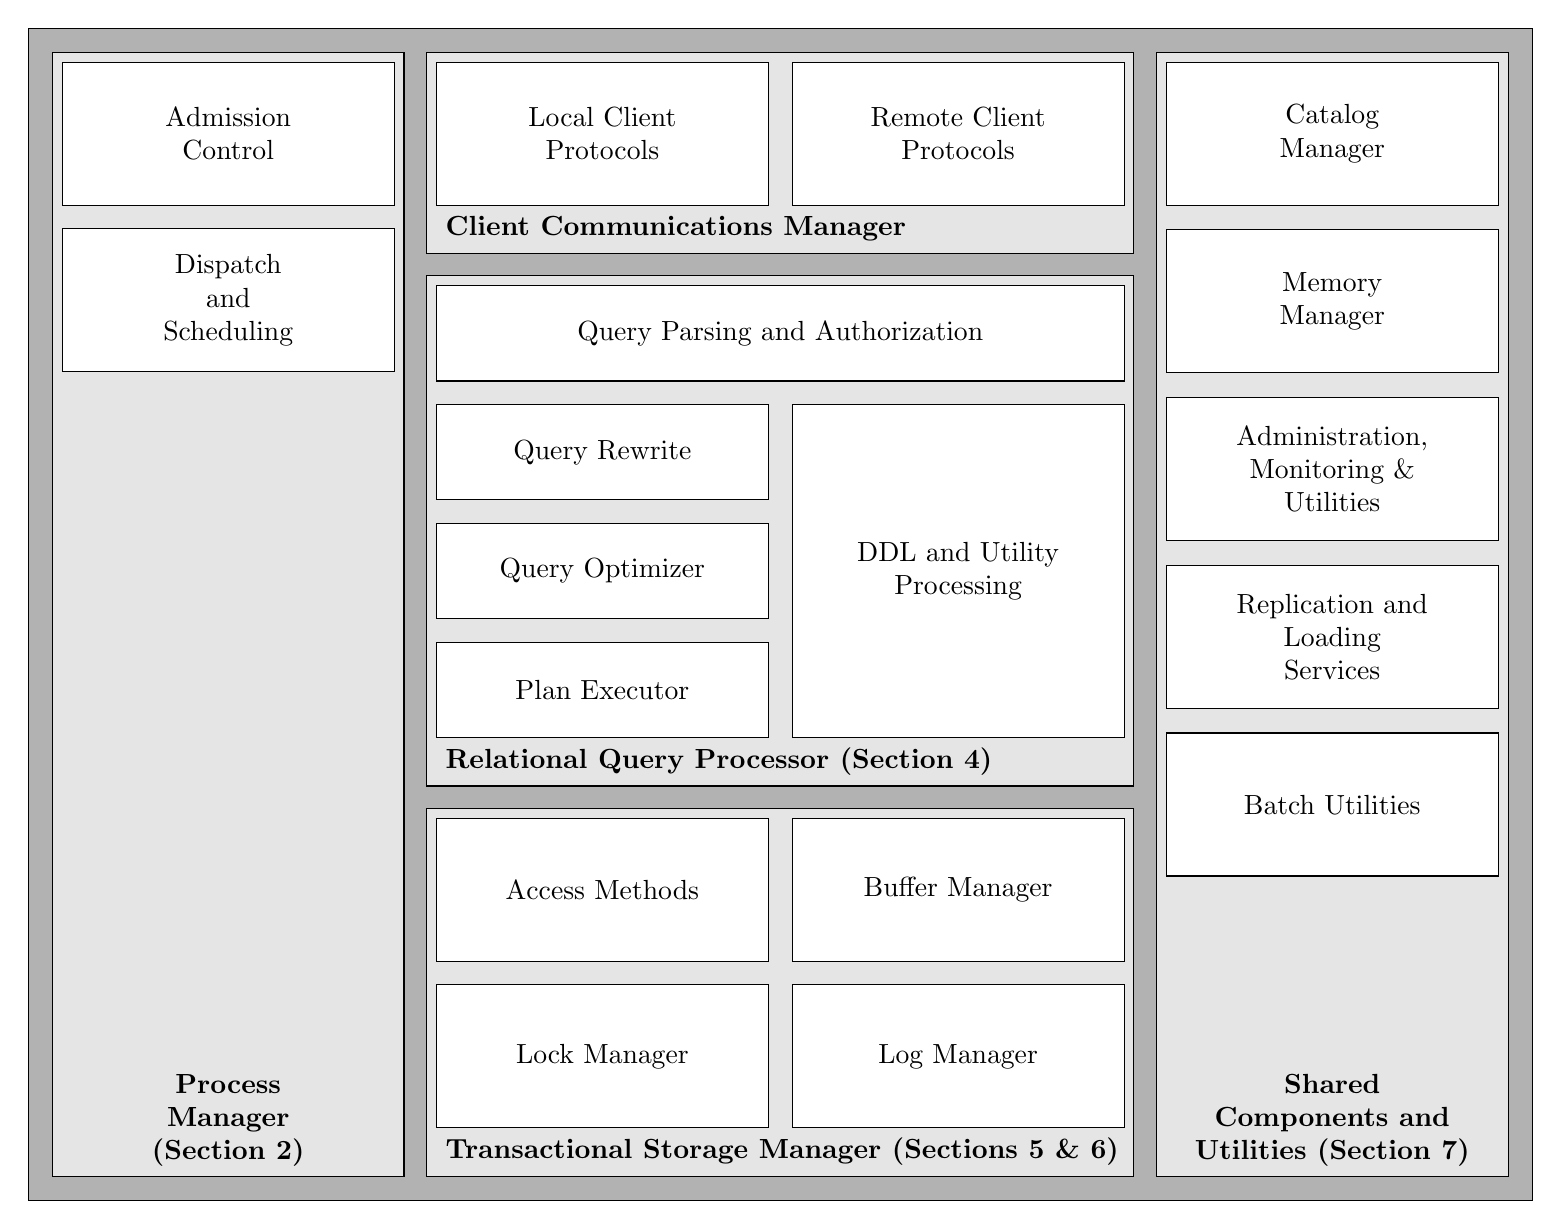
\begin{tikzpicture}[
  node distance=\fignodesep,
  title/.style={font=\bfseries,minimum height=\figtitleheight},
  box/.style={draw,minimum width=\fignodewidth,minimum height=\fignodeheight,align=center,fill=white},
  box2/.style={draw,minimum width=\fignodewidth,minimum height=\fignodesmallheight,align=center,fill=white},
]

%%%%%%%%%%%%%%%
% Left Part
%%%%%%%%%%%%%%%
\node (l1) [box] {Admission\\Control};
\node [box,below={\fignodeheight + \fignodesep of l1.west},anchor=west] {Dispatch\\and\\Scheduling};


%%%%%%%%%%%%%%%
% Center Part
%%%%%%%%%%%%%%%
% Center Top
\node (cl1) [
  box,
  right={\fignodewidth + 2*\figinnersep + \fignodesep of l1.north}, % Box width + 2 * boundary inner sep + 3mm
  anchor=north
] {Local Client\\Protocols};
\node (cr1) [box,right={\fignodewidth + \fignodesep of cl1.north},anchor=north] {Remote Client\\Protocols};
\node (ct1) [title,below={1/2*(\fignodeheight + \figtitleheight) of cl1.west},anchor=west] {Client Communications Manager};
\node [
  draw,fit=(cl1)(cr1)(ct1), % Draw boundary of center top part
  inner ysep={1/2*\figinnersep},yshift={1/2*\figinnersep} % Eliminate bottom inner y separation
] {};

%%%%%%%%%%%%%%%
% Center Middle
\node (c2) [
  box2,
  minimum width={2*\fignodewidth + \fignodesep}, % Span 2 column
  below={1/2*(\fignodesmallheight + \figtitleheight) + \figinnersep + \fignodesep of ct1.west}, % Extra 1 boundary inner sep, because the bottom inner sep is eliminated.
  anchor=west
] {Query Parsing and Authorization};

\node (cl2) [box2,below={\fignodesmallheight + \fignodesep of c2.west},anchor=west] {Query Rewrite};
\node (cl3) [box2,below={\fignodesmallheight + \fignodesep of cl2.west},anchor=west] {Query Optimizer};
\node (cl4) [box2,below={\fignodesmallheight + \fignodesep of cl3.west},anchor=west] {Plan Executor};

\node (cr2) [
  box2,
  minimum height={3*\fignodesmallheight + 2*\fignodesep},
  below={1/2*(\fignodesmallheight + 3*\fignodesmallheight + 2*\fignodesep) + \fignodesep of c2.east},
  anchor=east
] {DDL and Utility\\Processing};

\node (ct2) [
  title,
  below={1/2*(\fignodesmallheight + \figtitleheight) of cl4.west},
  anchor=west
] {Relational Query Processor (Section 4)};

\node [
  draw,fit=(c2)(ct2), % Draw boundary of center middle part
  inner ysep={1/2*\figinnersep},yshift={1/2*\figinnersep} % Eliminate bottom inner y separation
] {};

%%%%%%%%%%%%%%%
% Center Bottom
\node (cl5) [
  box,
  below={1/2*(\fignodeheight + \figtitleheight) + \figinnersep + \fignodesep of ct2.west}, % Extra 1 boundary inner sep, because the bottom inner sep is eliminated.
  anchor=west
] {Access Methods};
\node (cr5) [
  box,
  right={\fignodewidth + \fignodesep of cl5.north},
  anchor=north
] {Buffer Manager};
\node (cl6) [box,below={\fignodeheight + \fignodesep of cl5.west},anchor=west] {Lock Manager};
\node (cr6) [box,below={\fignodeheight + \fignodesep of cr5.east},anchor=east] {Log Manager};
\node (fct3) [
  title,align=left,
  below={1/2*(\fignodeheight + \figtitleheight) of cl6.west},
  anchor=west
] {Transactional Storage Manager (Sections 5 \& 6)};
\node (ct3) [
  minimum height=\figtitleheight,
  minimum width={2*\fignodewidth + \fignodesep},
  below={1/2*(\fignodeheight + \figtitleheight) of cl6.west},
  anchor=west
] {};

\node [
  draw,fit=(cl5)(cr5)(ct3), % Draw boundary of center bottom part
  inner ysep={1/2*\figinnersep},yshift={1/2*\figinnersep} % Eliminate bottom inner y separation
] {};


%%%%%%%%%%%%%%%
% Right Part
%%%%%%%%%%%%%%%
\node (r1) [
  box,
  right={\fignodewidth + 2*\figinnersep + \fignodesep of cr1.north}, % Box width + 2 * boundary inner sep + 3mm
  anchor=north
] {Catalog\\Manager};
\node (r2) [box,below=of r1] {Memory\\Manager};
\node (r3) [box,below=of r2] {Administration,\\Monitoring \&\\Utilities};
\node (r4) [box,below=of r3] {Replication and\\Loading\\Services};
\node (r5) [box,below=of r4] {Batch Utilities};


%%%%%%%%%%%%%%%
% Tricky Parts
%%%%%%%%%%%%%%%
% Left Part Title & Boundary
\node (lt) [
  minimum width=12em,
  title,align=center,
  left={1/2*(\fignodewidth + 2*\fignodewidth + \fignodesep) + 2*\figinnersep + \fignodesep of ct3.south}, % Box width + 2 * boundary inner sep + 3mm
  anchor=south
] {Process\\Manager\\(Section 2)};
\node (l) [
  draw,fit=(l1)(lt), % Draw boundary of left part
  inner ysep={1/2*\figinnersep},yshift={1/2*\figinnersep} % Eliminate bottom inner y separation
] {};

%%%%%%%%%%%%%%%
% Right Part Title & Boundary
\node (rt) [
  minimum width=12em,
  title,align=center,
  right={1/2*(\fignodewidth + 2*\fignodewidth + \fignodesep) + 2*\figinnersep + \fignodesep of ct3.south}, % Box width + 2 * boundary inner sep + 3mm
  anchor=south
] {Shared\\Components and\\Utilities (Section 7)};
\node (r) [
  draw,fit=(r1)(rt), % Draw boundary of right part
  inner ysep={1/2*\figinnersep},yshift={1/2*\figinnersep} % Eliminate bottom inner y separation
] {};

%%%%%%%%%%%%%%%
% Background
\begin{scope}[on background layer]
\node [draw,inner sep=\fignodesep,fill=black!30,fit=(l)(r)] {};

\end{scope}
\begin{scope}[on background layer]
\node [fill=black!10,fit=(l1)(lt),inner ysep={1/2*\figinnersep},yshift={1/2*\figinnersep}] {};
\node [fill=black!10,fit=(r1)(rt),inner ysep={1/2*\figinnersep},yshift={1/2*\figinnersep}] {};
\node [fill=black!10,fit=(cl1)(cr1)(ct1),inner ysep={1/2*\figinnersep},yshift={1/2*\figinnersep}] {};
\node [fill=black!10,fit=(c2)(ct2),inner ysep={1/2*\figinnersep},yshift={1/2*\figinnersep}] {};
\node [fill=black!10,fit=(cl5)(cr5)(ct3),inner ysep={1/2*\figinnersep},yshift={1/2*\figinnersep}] {};
\end{scope}

\end{tikzpicture}
\end{document}
